% Chapter 9

\chapter{Outlier Detection and Statistical Validation} % Main chapter title

\label{Chapter11} % For referencing the chapter elsewhere, use \ref{Chapter1} 

For this step, I'm going to be using encoded data, so that I'm able to apply the methods to all columns (since they are now numeric). Here is the DataFrame:

\begin{figure}[h]
    \centering
    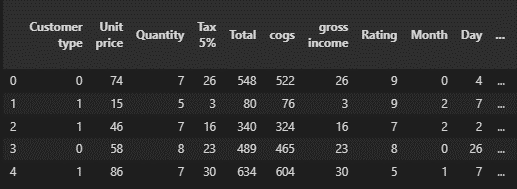
\includegraphics[width=1\textwidth]{Chapters/ch11/data_1.png}
    % \caption{This is an example image.}
    % \label{fig:example}
\end{figure}

\lhead{Chapter 11. \emph{Outlier Detection and Statistical Validation}} % This is for the header on each page - perhaps a shortened title

%----------------------------------------------------------------------------------------
Let’s consider the distinct value counts of all features, to get an idea of what we’re working with:

\begin{table}[htbp]
    \centering
    \begin{adjustbox}{max width=\textwidth} % Fit the table to the page width
        \rowcolors{1}{blue!20}{white} % Alternate row colors starting from the second row
        \rowcolors{2}{blue!30}{white} % Slightly darker header row
        \begin{tabular}{|>{\columncolor{blue!50}}c|c|}
            \hline
            \rowcolor{blue!50} % Slightly darker header row color
            \textbf{Customer type} & \textbf{Distinct Counts} \\
            \hline
            Unit price  & 90 \\
            Quantity  & 10 \\
            Tax 5\% & 49 \\
            Total & 546 \\
            COGS & 527 \\
            Gross income & 49 \\
            Rating & 7 \\
            Month & 3 \\
            Day & 31 \\
            Hour & 11 \\
            \verb|Branch_C| & 2 \\
            \verb|City_Naypyitaw| & 2\\
            \verb|City_Yangon| & 2 \\
            \verb|Gender_Male| & 2 \\
            \verb|Product line_Fashion accesories| & 2 \\
            \verb|Product line_Food and beverages| & 2 \\
            \verb|Product line_Health and beauty| & 2 \\
            \verb|Product line_Home and lifestyle| & 2 \\
            \verb|Product line_Sports and travel| & 2 \\
            \verb|Payment_Credit card| & 2 \\
            \verb|Payment_Ewallet| & 2 \\
            \hline
        \end{tabular}
    \end{adjustbox}
    % \caption{3 x 2 Table with alternating light green rows and a slightly darker green header}
    \label{tab:3x2_table}
\end{table}

All the encoded features have a distinct count of 2 since we used One-Hot encoding. Now, let’s move onto applying different methods for outlier detection.
% -----------------------------------------------------------------------------

\newpage
\section{Z-Score:}

\subsection{How does Z-Score work?}
\begin{equation}
Z = (X−mean)/std deviation
\end{equation}


The numerator $X - \mu$ calculates the difference between the individual data point ($X$) and the mean ($\mu$). This part of the formula measures how far the data point is from the center of the distribution. The result of the numerator is then divided by the standard deviation ($\sigma$). This division scales the difference in terms of standard deviations, providing a standardized measure of how far the data point is from the mean.

\newline 
A Z-score of 0 indicates that the data point's value is exactly at the mean. A positive Z-score indicates that the data point is above the mean, and the magnitude of the Z-score tells us how many standard deviations above the mean the data point is. A negative Z-score indicates that the data point is below the mean, and again, the magnitude represents how many standard deviations below the mean.

% -----------------------------------------------------------------------------------------------------------

\subsection{Applying Z-Score in code:}
In our code, we calculate the Z-score for each data point in selected columns of interest (e.g., Total, Unit price, Quantity) and identify outliers based on a user-defined threshold.

\lstset{language=Python}
\begin{lstlisting}
threshold_values = np.arange(1, 4, 0.5)
\end{lstlisting}

We must define a threshold value which will indicate the range for which we are considering the Z-score. The \verb|‘threshold_values’| is defined as an array ranging from 1 to 3. This array represents a range of threshold values that will be used in the outlier detection process.
\newline 
As well as this, we make use of ‘steps’ to identify outliers. The concept of using steps refers to the systematic exploration of different threshold values in the outlier detection process. Here, I made use of the Numpy function ‘arrange’ to define the number of steps, which I set at 0.5. Basically, the code will consider the dataset in increments of 0.5 (Threshold Value).
\newline 
The choice of starting from 1 and incrementing in steps of 0.5 allows for a nuanced exploration of outlier detection sensitivity. Lower thresholds may capture more points as outliers, while higher thresholds may only capture extreme anomalies.

% -------------------------------------------------------------------------------------------------------------------------------------------------------------------------------------------

\subsection{Result and Analysis:}

\definecolor{headercolor}{RGB}{255,128,0} % Define the header color (slightly darker orange)
\definecolor{rowcolor}{RGB}{255,218,185} % Define the row color (light orange)



\begin{table}[htbp]
\centering
\rowcolors{2}{rowcolor}{white} % Alternating row colors starting from the second row
\begin{adjustbox}{width=\textwidth}
\begin{tabular}{|c|c|c|c|c|c|c|c|c|}
\hline
\rowcolor{headercolor}
Threshold & Total & Customer type & Unit price & Quantity & Tax 5\% & Total & COGS & Gross Income \\
\hline
1.0 & 308 & 499 & 426 & 414 & 331 & 308 & 311 & 331 \\
1.5 & 112 & 0 & 139 & 231 & 112 & 112 & 112 & 112 \\
2.0 & 54 & 0 & 0 & 0 & 52 & 54 & 53 & 52 \\
2.5 & 17 & 0 & 0 & 0 & 11 & 17 & 17 & 11 \\
3.0 & 0 & 0 & 0 & 0 & 0 & 0 & 0 & 0 \\
3.5 & 0 & 0 & 0 & 0 & 0 & 0 & 0 & 0 \\
\hline
\end{tabular}
\end{adjustbox}
% \caption{A 7 by 9 table with alternating row colors}
\end{table}


As expected, increasing the threshold leads to a decrease in the number of identified outliers. At the highest threshold (3.5), no outliers are detected in any column, indicating a more conservative approach to outlier identification.

\begin{itemize}
\item Total: The 'Total' column consistently has a high number of outliers across different thresholds, suggesting potential anomalies in the overall sales amount.
\item Customer Type: The count of outliers for 'Customer type' is notably high at lower thresholds, indicating potential unusual patterns related to customer types.
\item Unit Price, Quantity, Tax 5\%: These columns show varying counts of outliers, suggesting potential discrepancies in pricing, purchase quantities, and tax amounts.
\item Rating: Outliers in the 'Rating' column decrease with higher thresholds, indicating that extreme ratings become less significant as the threshold increases.
\end{itemize}
\newline 
At certain thresholds, some columns have zero outliers. This is particularly evident for 'Hour' and 'Day,' which implies that these features might exhibit consistent patterns without significant outliers.


\begin{figure}[h]
    \centering
    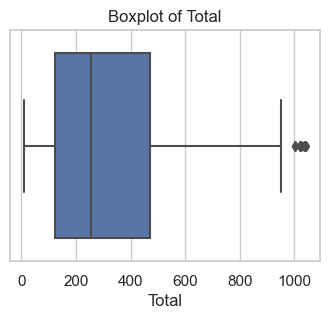
\includegraphics[width=0.5\textwidth]{Chapters/ch11/ch11_box_ploy_initial.png}
    % \caption{This is an example image.}
    % \label{fig:example}
\end{figure}

As can be observed, a certain number of outliers do seem to lie in the ‘Total’ column. 
\newline
I displayed all instances containing outliers in the column ‘Total’ and found these to be 17 rows in total.


\section{Interquartile Range:}
The Interquartile Range (IQR) is calculated as the difference between the third quartile (Q3) and the first quartile (Q1). This statistical measure is robust against extreme values and forms the basis for identifying outliers. The lower and upper bounds for potential outliers are established by extending 1.5 times the IQR below Q1 and above Q3, respectively. 
\newline
Upon applying this method, I obtained 9 outlier rows based on the ‘Total’ feature.

\begin{figure}[h]
    \centering
    \begin{subfigure}{0.5\textwidth}
        \centering
        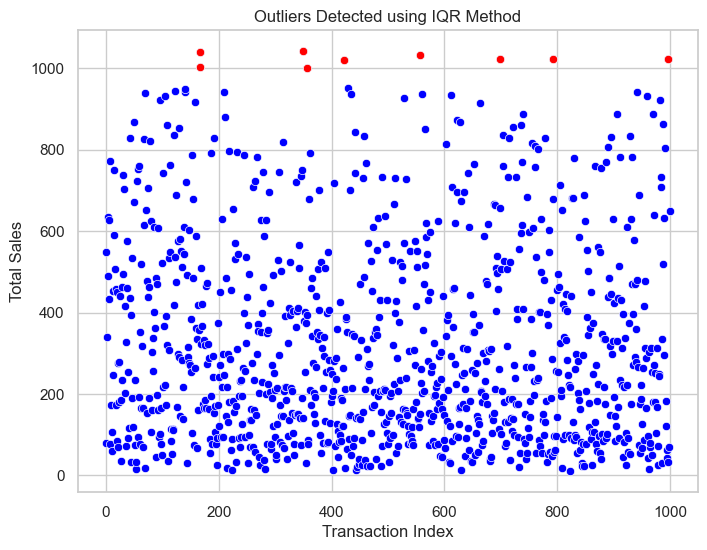
\includegraphics[width=\linewidth]{Chapters/ch11/ch_11_scatterplot.png}
        \caption{Scatterplot}
        \label{fig:scatterplot}
    \end{subfigure}%
    \begin{subfigure}{0.5\textwidth}
        \centering
        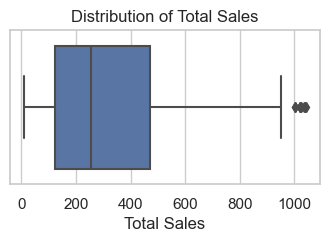
\includegraphics[width=\linewidth]{Chapters/ch11/ch_11_boxplot.png}
        \caption{Boxplot}
        \label{fig:boxplot}
    \end{subfigure}
    \caption{Two plots side by side}
    \label{fig:bothplots}
\end{figure}

% -----------------------------------------------------------------------------------------------
\newpage
\section{Isolation Forest:}
The Isolation Forest algorithm is a robust technique for identifying outliers or anomalies within a dataset, particularly adept at handling high-dimensional data efficiently. Its core concept revolves around the construction of isolation trees, binary trees that isolate data points by recursively partitioning the feature space. Anomalies, being rare instances, are expected to have shorter path lengths in these trees. The algorithm builds an ensemble of such trees and derives anomaly scores based on the average path length. Lower scores signify points that are easier to isolate and are thus more likely to be outliers.
\newline
The focus is on key dimensions such as 'Total', 'Unit price', 'Quantity', and 'cogs' columns, which are deemed crucial for understanding customer.
\newline 
\begin{lstlisting}[language=Python, frame=none]
model = IsolationForest(contamination=0.01)
\end{lstlisting}
\newline 
In the code above, a contamination parameter of 0.01 is set, indicating the proportion of outliers expected in the dataset. The Isolation Forest algorithm assigns an anomaly score to each data point, and those with a score indicative of an outlier (equal to -1) are isolated and extracted into a separate dataframe.
\newline 
A total of 10 rows are identified as outliers. Note that these are the top 1\% outliers in our dataset based on the following features: 'Total', 'Unit price', 'Quantity' and 'cogs'.
% -----------------------------------------------------------------------------------------------------------------------
\section{Statistical Validation:}
Statistical validation in the context of outlier detection involves applying formal statistical methods to assess and confirm the significance of identified outliers. It helps ensure that the patterns or anomalies observed in the data are not due to random chance and are, instead, statistically meaningful. The goal is to provide a robust foundation for drawing accurate conclusions from the detected outliers.

\subsection{ANOVA:}
Analysis of Variance is a statistical method used to compare means among multiple groups to determine if there are any statistically significant differences. It allows for the assessment of whether the variability within groups is comparable to the variability between groups. It is used to test the null hypothesis that there is no significant difference among the means of three or more groups. It also provides insights into whether any observed differences in means are likely due to genuine differences between groups or simply due to random variation.
\newline 
After making use of ANOVA in my code, I was unable to detect any significant patterns. Upon testing for both ‘Total’ and ‘Customer type’ features, I found no significant difference amongst the different categories of both features. This was indicated to me by the values of T-statistic and P-value, which ANOVA calculates. 

\subsection{Hypothesis Testing:}
In statistical validation, we often formulate hypotheses regarding the presence of outliers or patterns in the data.
\begin{itemize}
    \item Null Hypothesis (H0): Assumes that there are no significant outliers or patterns.
    \item Alternative Hypothesis (H1): Assumes the presence of significant outliers or patterns.
\end{itemize}
Hence in our case, the Null Hypothesis would be that there is no significant difference in total sales between normal transactions and outliers. And the Alternative Hypothesis would be that there is a significant difference in total sales between normal transactions and outliers.

\subsubsection{Two-Sample t-Test:}
\begin{itemize}
    \item T-Statistic: This measures the difference between the means of the two groups relative to the variability within each group. A higher absolute t-statistic suggests a greater difference between the groups.
    \item P-Value: The p-value represents the probability of obtaining the observed results (or more extreme) under the assumption that the null hypothesis is true. A lower p-value indicates stronger evidence against the null hypothesis.
\end{itemize}
So, in our case, the computed t-statistic is a quantitative measure of the difference in total sales between normal transactions and outliers. And our P-Value will indicate whether there is a significant difference in total sales. If there is, we will reject the null hypothesis.
\newline 
The significance level is denoted by alpha (α). This chosen level represents the threshold below which we would reject the null hypothesis. A common practice is to set alpha at 0.05, indicating a 5\% probability of rejecting the null hypothesis when it is true. Hence, I also set it at 0.05.

\begin{center}
\begin{tabular}{|c|c|}
\hline
\rowcolor{green!20} \textbf{T-Statistic} & \textbf{8.916895886005445} \\
\hline
\cellcolor{green!10} \textbf{P-Value} & \textbf{2.2421883966112505e-18} \\
\hline
\end{tabular}
\end{center}

With a p-value much smaller than the significance level, we reject the null hypothesis. Therefore, we conclude that there is a significant difference in total sales between normal transactions and outliers in our dataset.
\newline
The negative t-statistic indicates that outliers tend to have lower mean total sales compared to normal transactions. 



